\documentclass[]{article}

% Imported Packages
%------------------------------------------------------------------------------
\usepackage{amssymb}
\usepackage{amstext}
\usepackage{amsthm}
\usepackage{amsmath}
\usepackage{enumerate}
\usepackage{fancyhdr}
\usepackage[margin=1in]{geometry}
\usepackage{graphicx}
\usepackage{extarrows}
\usepackage{setspace}
%------------------------------------------------------------------------------

% Header and Footer
%------------------------------------------------------------------------------
\pagestyle{plain}  
\renewcommand\headrulewidth{0.4pt}                                      
\renewcommand\footrulewidth{0.4pt}                                    
%------------------------------------------------------------------------------

% Title Details
%------------------------------------------------------------------------------
\title{Deliverable \#3 Template}
\author{SE 3A04: Software Design II -- Large System Design}
\date{}                               
%------------------------------------------------------------------------------

% Document
%------------------------------------------------------------------------------
\begin{document}

\maketitle	

\section{Introduction}
\label{sec:introduction}
% Begin Section

%This section should provide an brief overview of the entire document.

\subsection{Purpose}
\label{sub:purpose}
% Begin SubSection
%\begin{enumerate}[a)]
%	\item Delineate the purpose of the document
%	\item Specify the intended audience for the document
%\end{enumerate}
% End SubSection
The purpose of this document is to give a more detailed look as to how the system is connected. The intended audience are IT professionals, the TAs and professor, 
\subsection{System Description}
\label{sub:system_description}
% Begin SubSection
%\begin{enumerate}[a)]
%	\item Give a brief description of the system. This could be a paragraph or two to give some context to this document.
%\end{enumerate}
The system that is being build 
% End SubSection

\subsection{Overview}
\label{sub:overview}
% Begin SubSection
%\begin{enumerate}[a)]
%	\item Describe what the rest of the document contains 
%	\item Explain how the document is organised
%\end{enumerate}
This document contains the state charts for all controller classes, all sequence diagrams, and a detailed class diagram. Section two of this document contains the state charts for the User Interface Controller, the Expert Controller, and the Experts. There will be six state charts, each corresponding to one controller. Section three consists of the sequence diagrams, and finally section four is focused on detailed class diagrams. This section will break down each class into methods, variables, and how each class interacts with each other. 
% End SubSection

% End Section

\section{State Charts for Controller Classes}
\label{sec:state_charts_for_controller_classes}
% Begin Section
This section should provide a state chart for each controller class for your application.
% End Section

\section{Sequence Diagrams}
\label{sec:sequence_diagrams}
% Begin Section
****help insert images!!!!*****
\begin{figure}[!hb]
	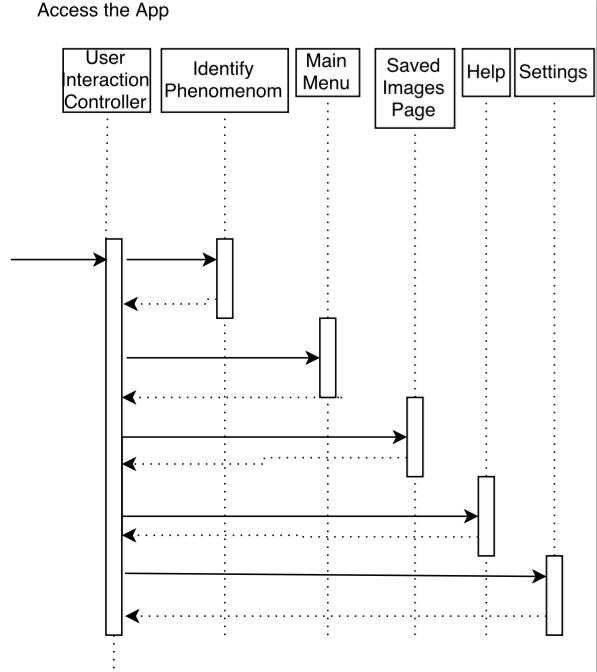
\includegraphics[width=\linewidth]{sequenceDiagram1.png}
	\caption{Sequence Diagram for Accessing the Application}
\end{figure}
\begin{figure}[!hb]
	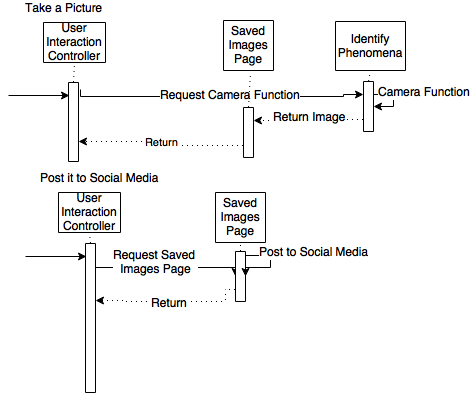
\includegraphics[width=\linewidth]{sequenceDiagram2.png}
	\caption{Sequence Diagram for Taking a Picture and Posting it to Social Media}
\end{figure}
\begin{figure}[!hb]
	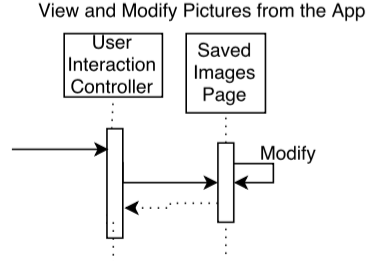
\includegraphics[width=\linewidth]{sequenceDiagram3.png}
	\caption{Sequence Diagram for Viewing and Modifying Pictures from the Application}
\end{figure}
\begin{figure}[!hb]
	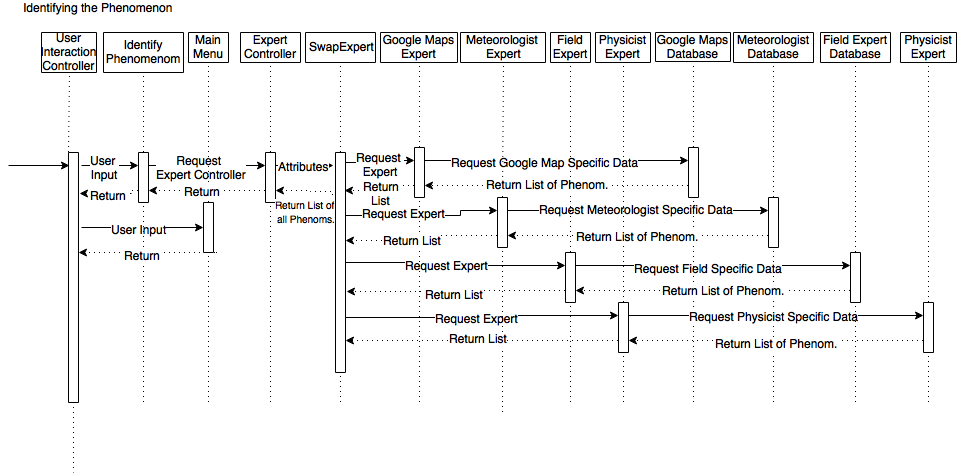
\includegraphics[width=\linewidth]{sequenceDiagram4.png}
	\caption{Sequence Diagram for Identifying the Phenomenon}
\end{figure}

% End Section

\section{Detailed Class Diagram}
\label{sec:detailed_class_diagram}
% Begin Section
This section should provide a detailed class diagram for your application.
% End Section

\appendix
\section{Division of Labour}
\label{sec:division_of_labour}
% Begin Section
Include a Division of Labour sheet which indicates the contributions of each team member. This sheet must be signed by all team members.
% End Section

\newpage
\section*{IMPORTANT NOTES}
\begin{itemize}
	\item You do \underline{NOT} need to provide a text explanation of each diagram; the diagram should speak for itself
	\item Please document any non-standard notations that you may have used
	\begin{itemize}
		\item \emph{Rule of Thumb}: if you feel there is any doubt surrounding the meaning of your notations, document them
	\end{itemize}
	\item Some diagrams may be difficult to fit into one page
	\begin{itemize}
		\item It is OK if the text is small but please ensure that it is readable when printed
		\item If you need to break a diagram onto multiple pages, please adopt a system of doing so and throughly explain how it can be reconnected from one page to the next; if you are unsure about this, please ask me
	\end{itemize}
	\item Please submit the latest version of Deliverable 1 and Deliverable 2 with Deliverable 3
	\begin{itemize}
		\item They do not have to be a freshly printed versions; the latest marked versions are OK
	\end{itemize}
	\item If you do \underline{NOT} have a Division of Labour sheet, your deliverable will \underline{NOT} be marked
\end{itemize}


\end{document}
%------------------------------------------------------------------------------